\section{Results}

All values in this section are generated from the aggregate CSV summary produced by the pipeline. The three main examples compare local Langevin, raw compound-Poisson (CP), and the L\'evy-score-corrected CP (LSC-CP); the benchmark additionally reports MALA, BAOAB, HMC, and PT. Efficiency numbers (ESS/sec) are always reported alongside a target-fidelity error, because a non-converged sampler can post a high ESS on the wrong distribution.

\subsection{Quantitative summary}

\begin{itemize}
\item Double well: LSC-CP reduces the CDF-sup target error from 0.109 (raw CP) to 0.020, a genuine invariant-measure correction (Fig.~timestep-bias shows this defect is timestep-independent).
\item 10D transformed M\"uller--Brown: LSC-CP with lifted basin-to-basin jumps attains basin-TV 0.012 versus 0.181 for raw CP and beats a random-direction matched-length control (0.124).
\item Triple well: the stationary correction keeps mode-TV small for both supports (overlong 0.015, adjacent 0.047); support choice governs which modes communicate directly.
\item Started at equilibrium, LSC-CP preserves the target (basin-TV 0.012) while raw CP drifts off it (0.191).
\item ManyWell high-D stress test: lowest block-marginal KL is 8.58e-04 for LSC-CP/manywell\_block\_flip on manywell\_d8.
\end{itemize}


\subsection{Double well: target fidelity}With a shared shell jump law, LSC-CP attains CDF-sup error 0.020 versus 0.109 for raw CP and 0.402 for local Langevin (which stays near its metastable initial well over the displayed horizon). The timestep-bias study confirms the raw-CP error is independent of the integrator step, i.e.\ a genuine change of invariant law rather than a discretization artifact.

\subsection{Triple well: support versus bias}Corrected adjacent and overlong supports both keep mode-TV small (0.047 and 0.015), while the uncorrected overlong control records the bias of omitting the correction (0.168). A too-short shell (mode-TV 0.375) fails to connect the modes and behaves like local noise. The correction governs target fidelity; the support governs which modes communicate directly.

\subsection{Transformed M\"uller--Brown (10D)}After lifting the latent-minima displacements through the mixing map, LSC-CP attains basin-TV 0.012 versus 0.181 for raw CP, 0.124 for a random-direction matched-length control, and 0.110 for local Langevin. Acceleration therefore comes specifically from geometry-matched inter-basin jumps, not from nonlocal jumps of the same length in arbitrary directions.

\subsection{Efficiency benchmark}On the smooth low-dimensional double well, LSC-CP is the most accurate (CDF-sup 0.020) but not the fastest per wall-clock (ESS/sec 3311.803) because of the L\'evy-score quadrature. Local Langevin posts a far higher ESS/sec (17105.489) at a much larger bias (0.402), illustrating why ESS must be read together with target fidelity. The method's efficiency advantage appears in the trapped and high-dimensional regimes (four well, ManyWell).

\subsection{Additional landscapes}Four-well graph ablation: lowest basin KL 0.002 for raw CP/minima\_complete\_graph. Structured geometry-matched jumps beat the random matched-length control (0.002 vs.\ 0.018).

ManyWell high-dimensional stress test: lowest block-marginal KL 8.58e-04 for LSC-CP/manywell\_block\_flip on manywell\_d8, the regime where local samplers remain entropically confined and the block-flip jumps match the product structure.

\subsection{Alanine dipeptide (Ramachandran torus)}On an analytic surrogate for the alanine-dipeptide free-energy surface (a periodic mixture over the conformational basins), wrapped basin-to-basin jumps give LSC-CP the best basin-population fidelity (basin-TV 0.013, all-basin coverage fraction 0.976), versus 0.027 for a random-direction control, 0.174 for uncorrected raw CP, and 0.387 for local Langevin (which stays confined to its starting basin). Parallel tempering is the only baseline that competes on coverage. The construction extends unchanged to the torus via wrapped displacements and a periodic score.

\subsection{Lennard-Jones cluster: a structural limitation}For an LJ$_{7}$ cluster in two dimensions the fixed Cartesian jump bank is incompatible with the cluster's continuous rotational symmetry. A jump aligned in the catalogue frame is productive only while the cluster keeps that orientation: sweeping the cluster orientation, the fixed jump lands at low (isomer) energy for only 2.740\% of angles before running into hard-core overlaps, whereas a rotationally-augmented gated bank (rotated copies of the jump, gated by landing energy) restores productivity to 100.000\%. This delineates the method's scope: fixed additive jumps suit targets whose metastable transitions are fixed coordinate displacements, not systems with continuous symmetries.

\subsection{LJ$_{38}$ double funnel: barrier limitation and a darting hybrid}The canonical metastable cluster is LJ$_{38}$, whose FCC truncated-octahedron global minimum (-173.928, recovered exactly) competes with an icosahedral funnel (-170.990). The straight-line displacement between the two funnels crosses a 87.700~$\varepsilon$ barrier of atomic overlaps, so at the solid--solid transition temperature $\beta\cdot$barrier~$\approx728$ and the rejection-free score integrand $\exp[-\beta\,\Delta V]$ is numerically zero: the additive correction \emph{cannot} make a barrier-crossing jump target-preserving. The same geometry-matched inter-funnel displacement, applied as a \emph{Metropolis-corrected} endpoint dart (accept on the endpoint energy, no path integral), escapes the icosahedral funnel and reaches the FCC global (FCC-funnel fraction from the icosahedral start: local MC 0.000 vs darting 1.000). Thus geometry-matched nonlocal jumps solve the LJ$_{38}$ global-funnel-discovery problem, but through the Metropolis-corrected hybrid rather than the pure additive score; recovering the entropy-balanced funnel populations at the transition needs the full smart-darting machinery (darting regions and Jacobians), which we leave to future work.

\subsection{Generated figures}
\begin{figure}[t]
\centering
\begin{minipage}{0.48\textwidth}
\centering
\IfFileExists{figures/fig_dw_cdf_sup.pdf}{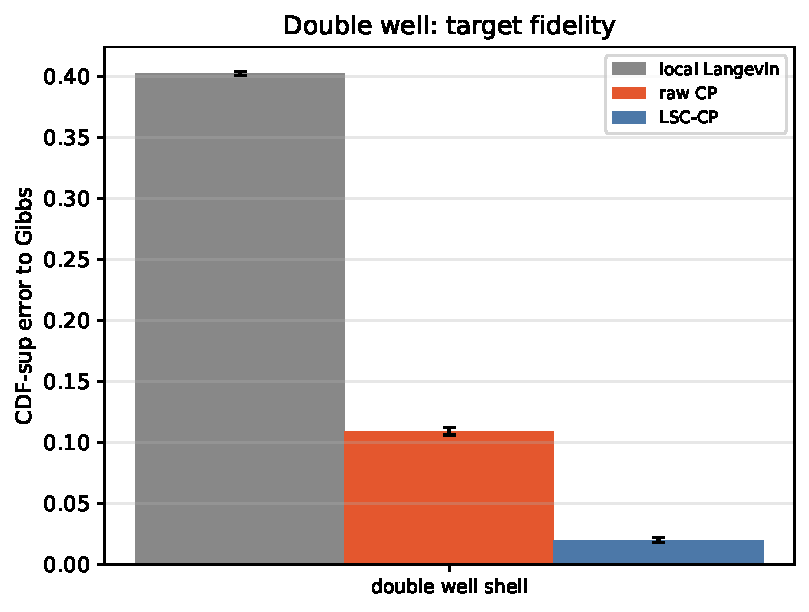
\includegraphics[width=\textwidth]{figures/fig_dw_cdf_sup.pdf}}{}
\caption*{Double well: target fidelity (CDF-sup)}
\end{minipage}
\hfill
\begin{minipage}{0.48\textwidth}
\centering
\IfFileExists{figures/fig_dw_density_l1.pdf}{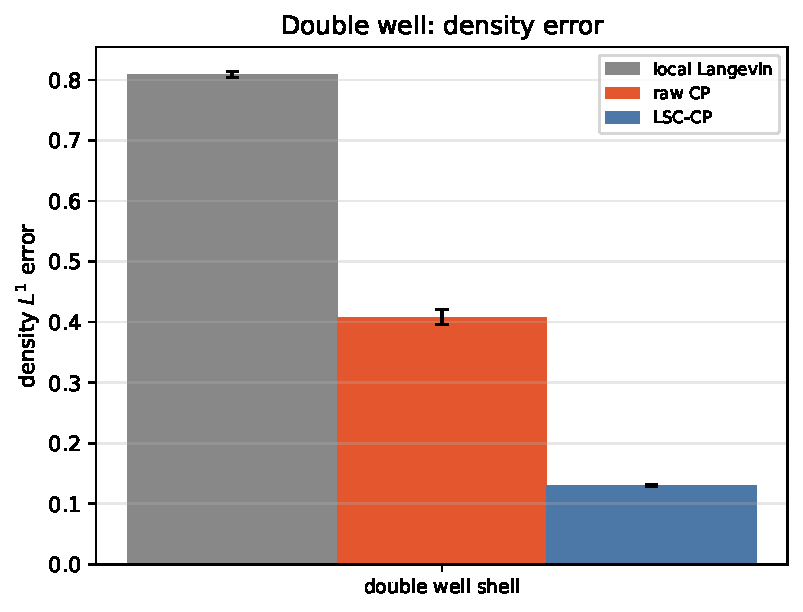
\includegraphics[width=\textwidth]{figures/fig_dw_density_l1.pdf}}{}
\caption*{Double well: density $L^1$ error}
\end{minipage}
\caption{Generated manuscript figure(s) 1--2 from aggregate CSV summaries.}
\label{fig:generated-1}
\end{figure}
\begin{figure}[t]
\centering
\begin{minipage}{0.48\textwidth}
\centering
\IfFileExists{figures/fig_timestep_bias.pdf}{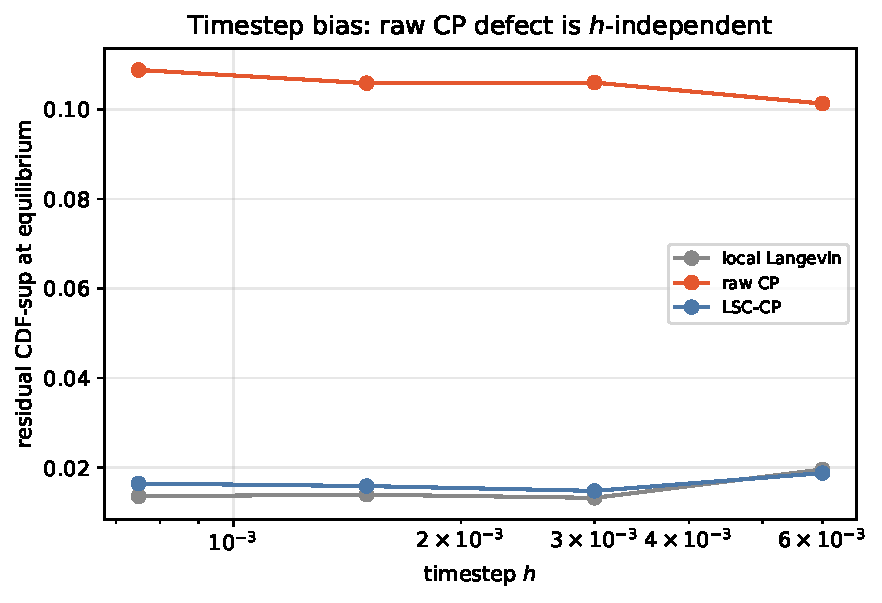
\includegraphics[width=\textwidth]{figures/fig_timestep_bias.pdf}}{}
\caption*{Timestep bias: raw CP defect is $h$-independent}
\end{minipage}
\hfill
\begin{minipage}{0.48\textwidth}
\centering
\IfFileExists{figures/fig_scale_intensity_relax.pdf}{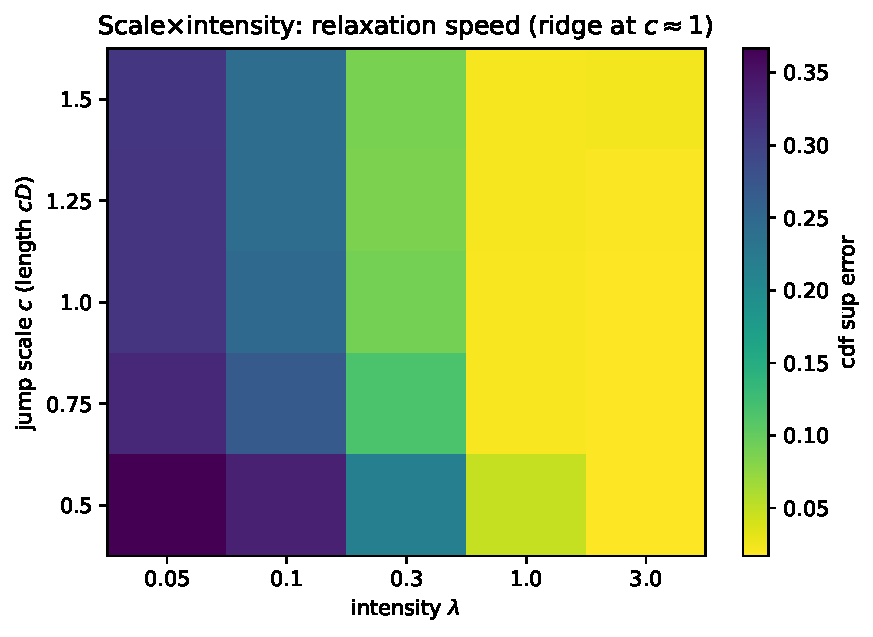
\includegraphics[width=\textwidth]{figures/fig_scale_intensity_relax.pdf}}{}
\caption*{Scale$\textbackslash\{\}times$intensity relaxation ridge}
\end{minipage}
\caption{Generated manuscript figure(s) 3--4 from aggregate CSV summaries.}
\label{fig:generated-2}
\end{figure}
\begin{figure}[t]
\centering
\begin{minipage}{0.48\textwidth}
\centering
\IfFileExists{figures/fig_tw_mode_tv.pdf}{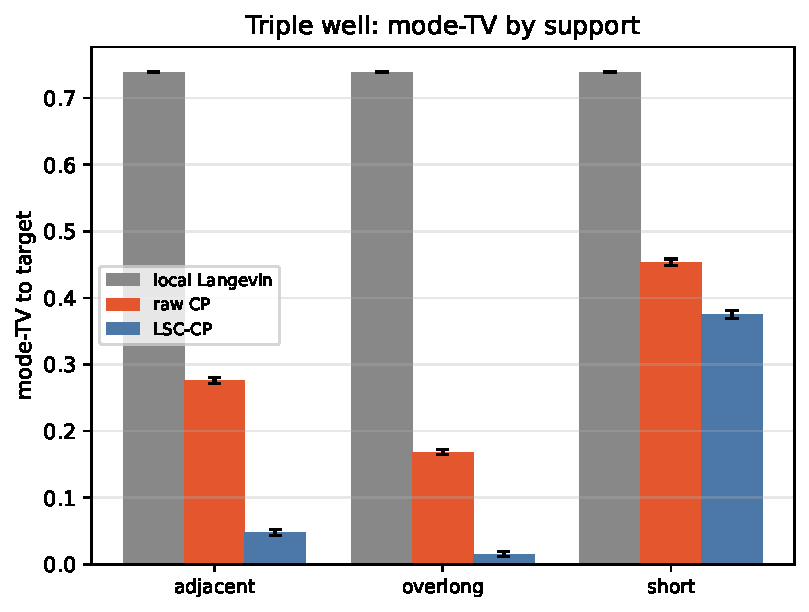
\includegraphics[width=\textwidth]{figures/fig_tw_mode_tv.pdf}}{}
\caption*{Triple well: mode-TV by support}
\end{minipage}
\hfill
\begin{minipage}{0.48\textwidth}
\centering
\IfFileExists{figures/fig_tw_middle_mass.pdf}{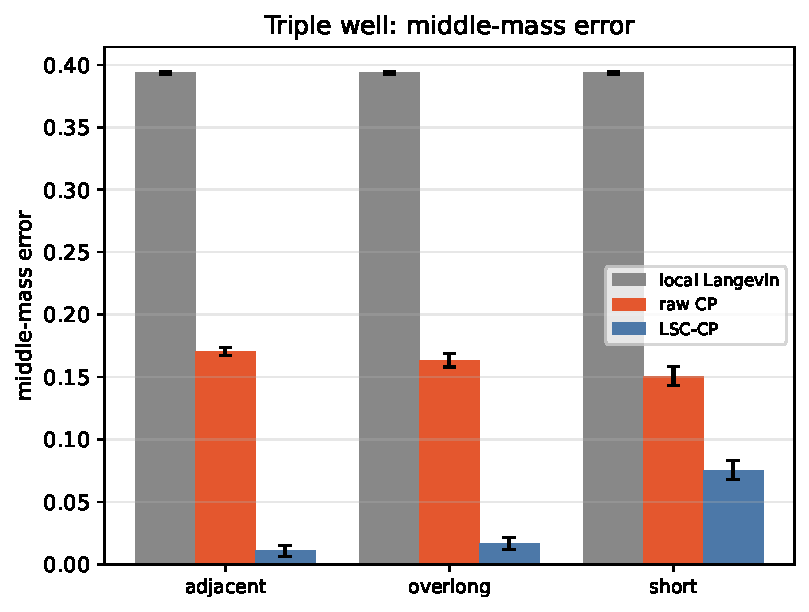
\includegraphics[width=\textwidth]{figures/fig_tw_middle_mass.pdf}}{}
\caption*{Triple well: middle-mass error}
\end{minipage}
\caption{Generated manuscript figure(s) 5--6 from aggregate CSV summaries.}
\label{fig:generated-3}
\end{figure}
\begin{figure}[t]
\centering
\begin{minipage}{0.48\textwidth}
\centering
\IfFileExists{figures/fig_mb10_basin_tv.pdf}{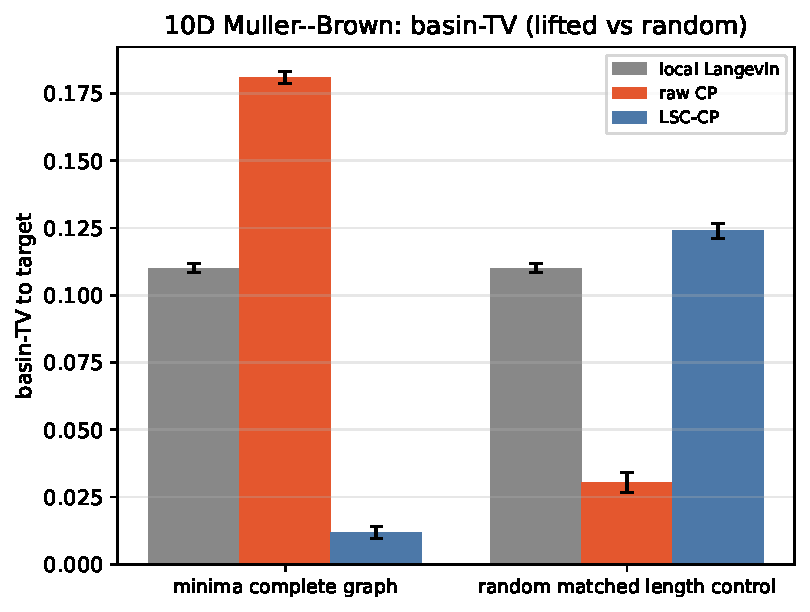
\includegraphics[width=\textwidth]{figures/fig_mb10_basin_tv.pdf}}{}
\caption*{10D Muller--Brown: basin-TV (lifted vs random)}
\end{minipage}
\hfill
\begin{minipage}{0.48\textwidth}
\centering
\IfFileExists{figures/fig_invariance.pdf}{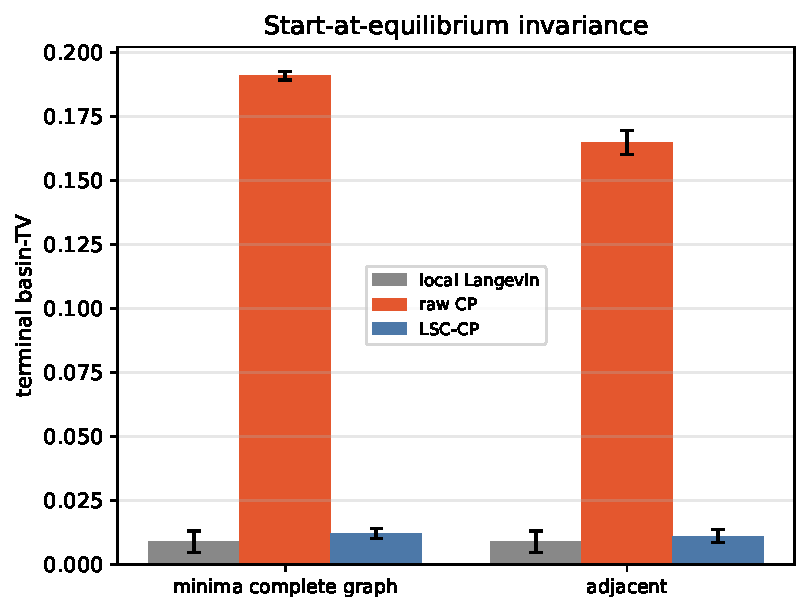
\includegraphics[width=\textwidth]{figures/fig_invariance.pdf}}{}
\caption*{Start-at-equilibrium invariance}
\end{minipage}
\caption{Generated manuscript figure(s) 7--8 from aggregate CSV summaries.}
\label{fig:generated-4}
\end{figure}
\begin{figure}[t]
\centering
\begin{minipage}{0.48\textwidth}
\centering
\IfFileExists{figures/fig_four_well_basin_kl.pdf}{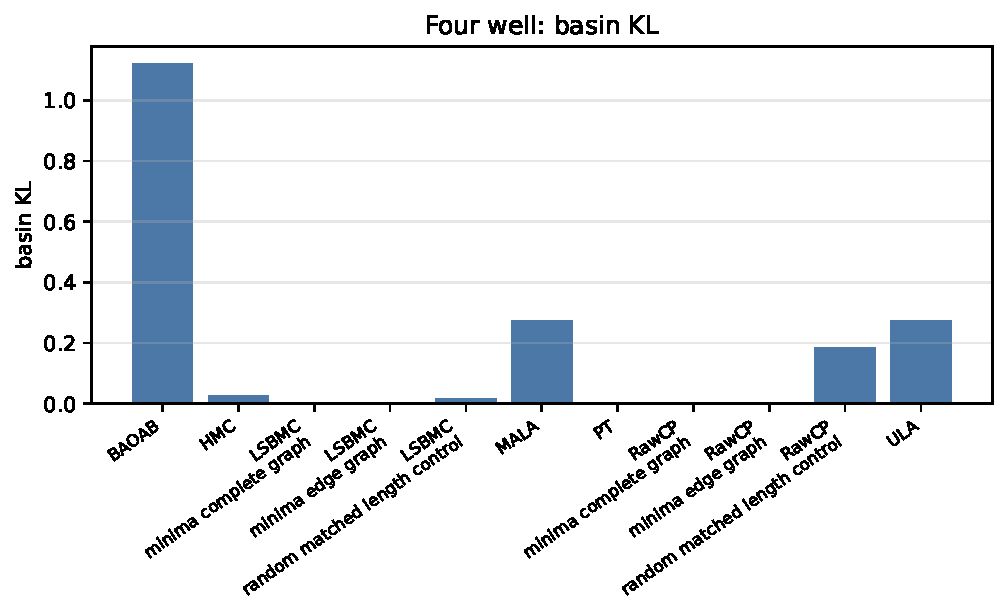
\includegraphics[width=\textwidth]{figures/fig_four_well_basin_kl.pdf}}{}
\caption*{Four-well graph ablation}
\end{minipage}
\hfill
\begin{minipage}{0.48\textwidth}
\centering
\IfFileExists{figures/fig_manywell_block_kl.pdf}{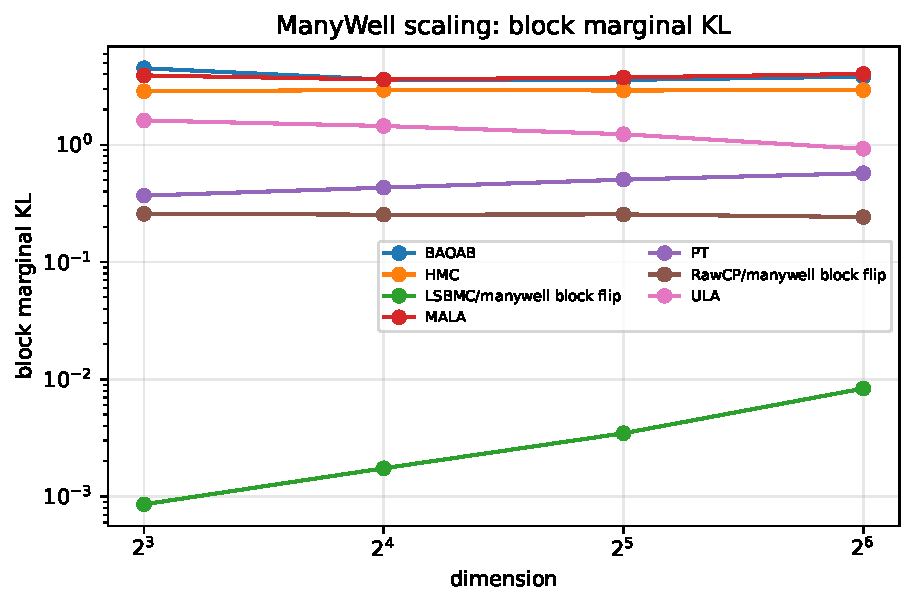
\includegraphics[width=\textwidth]{figures/fig_manywell_block_kl.pdf}}{}
\caption*{ManyWell block-marginal KL scaling}
\end{minipage}
\caption{Generated manuscript figure(s) 9--10 from aggregate CSV summaries.}
\label{fig:generated-5}
\end{figure}
\begin{figure}[t]
\centering
\begin{minipage}{0.48\textwidth}
\centering
\IfFileExists{figures/fig_alanine_basin_tv.pdf}{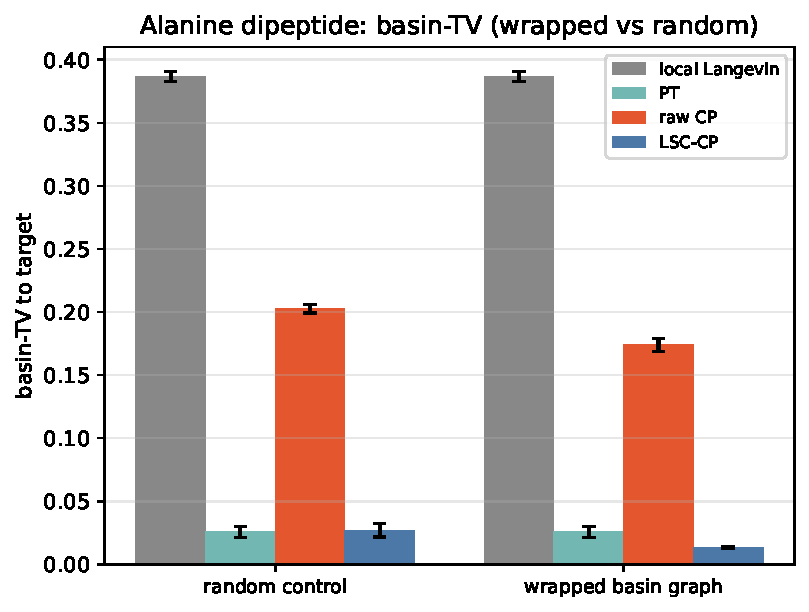
\includegraphics[width=\textwidth]{figures/fig_alanine_basin_tv.pdf}}{}
\caption*{Alanine dipeptide: basin-TV (wrapped vs random)}
\end{minipage}
\hfill
\begin{minipage}{0.48\textwidth}
\centering
\IfFileExists{figures/fig_lj_obstruction.pdf}{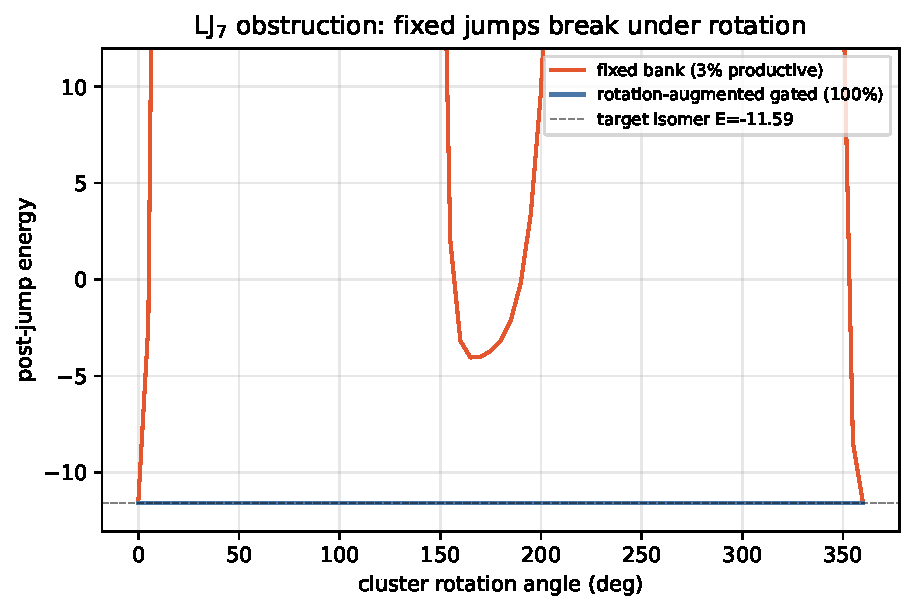
\includegraphics[width=\textwidth]{figures/fig_lj_obstruction.pdf}}{}
\caption*{Lennard-Jones rotational-symmetry obstruction}
\end{minipage}
\caption{Generated manuscript figure(s) 11--12 from aggregate CSV summaries.}
\label{fig:generated-6}
\end{figure}
\begin{figure}[t]
\centering
\begin{minipage}{0.48\textwidth}
\centering
\IfFileExists{figures/fig_lj38_darting.pdf}{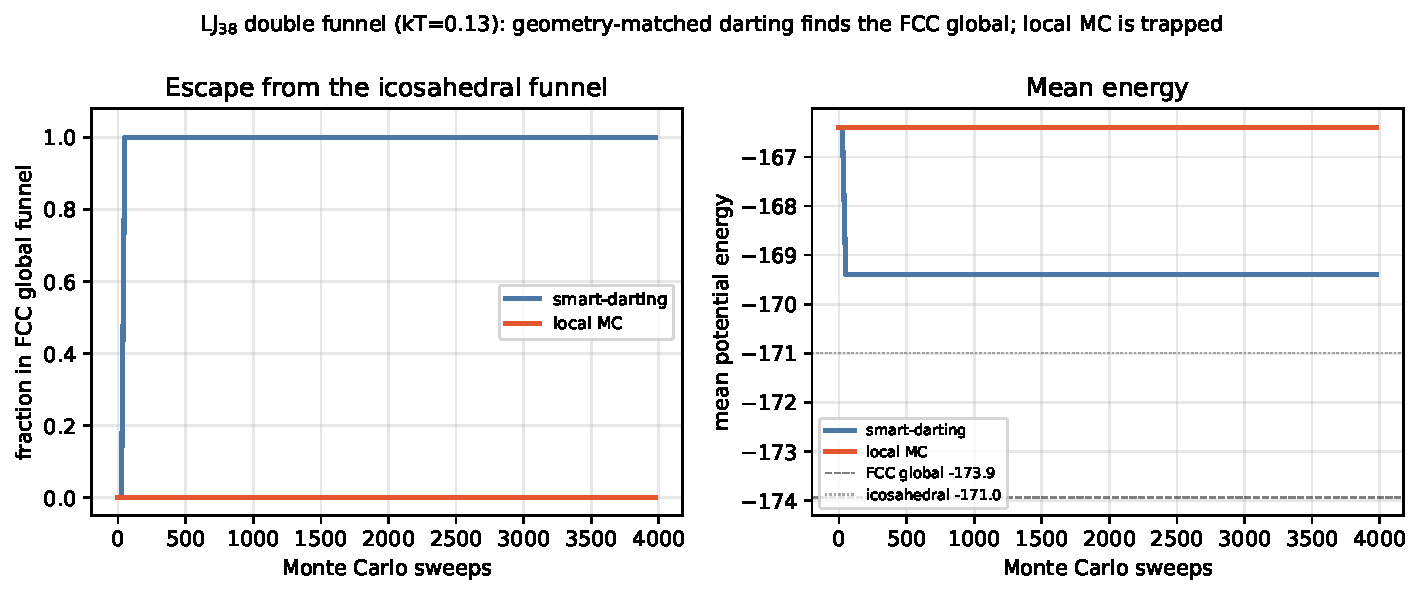
\includegraphics[width=\textwidth]{figures/fig_lj38_darting.pdf}}{}
\caption*{LJ38 double funnel: geometry-matched darting vs local MC}
\end{minipage}
\caption{Generated manuscript figure(s) 13 from aggregate CSV summaries.}
\label{fig:generated-7}
\end{figure}

\subsection{Generated tables}

\begin{table}[t]
\centering
\small
\caption{Generated metrics for alanine ramachandran. Means and standard errors are computed from raw CSV rows.}
\label{tab:alanine-ramachandran}
\resizebox{\textwidth}{!}{%
\begin{tabular}{llllrrrr}
\toprule
Target & Method & Bank & $n$ & basin-TV & FE RMSE & coverage frac & ESS/sec \\
\midrule
alanine\_torus & HMC & none & 4 & 0.186 & 0.187 & 0.176 & 87.650 \\
alanine\_torus & LSC-CP & random\_control & 4 & 0.027 & 0.157 & 0.984 & 608.963 \\
alanine\_torus & LSC-CP & wrapped\_basin\_graph (scale 1.0) & 4 & 0.013 & 0.147 & 0.976 & 493.708 \\
alanine\_torus & MALA & none & 4 & 0.292 & 0.145 & 0.038 & 378.413 \\
alanine\_torus & PT & none & 4 & 0.026 & 0.162 & 0.997 & 383.913 \\
alanine\_torus & raw CP & random\_control & 4 & 0.203 & 0.308 & 0.990 & 1154.724 \\
alanine\_torus & raw CP & wrapped\_basin\_graph (scale 1.0) & 4 & 0.174 & 0.284 & 0.989 & 1111.789 \\
alanine\_torus & local & none & 4 & 0.387 & 0.139 & 0.003 & 2259.066 \\
\bottomrule
\end{tabular}%
}
\end{table}
\begin{table}[t]
\centering
\small
\caption{Generated metrics for double well benchmark. Means and standard errors are computed from raw CSV rows.}
\label{tab:double-well-benchmark}
\resizebox{\textwidth}{!}{%
\begin{tabular}{llllrrrr}
\toprule
Target & Method & Bank & $n$ & CDF-sup & ESS/sec & ESS/grad & runtime (s) \\
\midrule
double\_well & BAOAB & none & 4 & 0.417 & 19342.155 & 3.824 & 0.317 \\
double\_well & HMC & none & 4 & 0.023 & 6353.787 & 0.671 & 1.014 \\
double\_well & LSC-CP & double\_well\_shell (scale 1.0) & 4 & 0.020 & 3311.803 & 4.737 & 2.289 \\
double\_well & MALA & none & 4 & 0.126 & 8046.389 & 1.869 & 0.743 \\
double\_well & PT & none & 4 & 0.070 & 6790.331 & 0.496 & 0.935 \\
double\_well & raw CP & double\_well\_shell (scale 1.0) & 4 & 0.109 & 7021.928 & 4.349 & 0.993 \\
double\_well & local & none & 4 & 0.402 & 17105.489 & 3.602 & 0.344 \\
\bottomrule
\end{tabular}%
}
\end{table}
\begin{table}[t]
\centering
\small
\caption{Generated metrics for double well reproduction. Means and standard errors are computed from raw CSV rows.}
\label{tab:double-well-reproduction}
\resizebox{\textwidth}{!}{%
\begin{tabular}{llllrrrr}
\toprule
Target & Method & Bank & $n$ & CDF-sup & density $L^1$ & coverage time & ESS/sec \\
\midrule
double\_well & LSC-CP & double\_well\_shell (scale 1.0) & 4 & 0.020 & 0.130 & 1.468 & 3443.816 \\
double\_well & raw CP & double\_well\_shell (scale 1.0) & 4 & 0.109 & 0.408 & 1.523 & 7378.841 \\
double\_well & local & none & 4 & 0.402 & 0.809 & 2.709 & 18125.156 \\
\bottomrule
\end{tabular}%
}
\end{table}
\begin{table}[t]
\centering
\small
\caption{Generated metrics for double well scale intensity. Means and standard errors are computed from raw CSV rows.}
\label{tab:double-well-scale-intensity}
\resizebox{\textwidth}{!}{%
\begin{tabular}{llllr}
\toprule
Target & Method & Bank & $n$ & ESS/sec \\
\midrule
double\_well & LSC-CP & c0.5\_l0.05 (scale 0.5) & 3 & 5463.796 \\
double\_well & LSC-CP & c0.5\_l0.1 (scale 0.5) & 3 & 5083.222 \\
double\_well & LSC-CP & c0.5\_l0.3 (scale 0.5) & 3 & 5349.143 \\
double\_well & LSC-CP & c0.5\_l1.0 (scale 0.5) & 3 & 7125.489 \\
double\_well & LSC-CP & c0.5\_l3.0 (scale 0.5) & 3 & 7632.834 \\
double\_well & LSC-CP & c0.75\_l0.05 (scale 0.75) & 3 & 7845.940 \\
double\_well & LSC-CP & c0.75\_l0.1 (scale 0.75) & 3 & 6206.249 \\
double\_well & LSC-CP & c0.75\_l0.3 (scale 0.75) & 3 & 6797.800 \\
double\_well & LSC-CP & c0.75\_l1.0 (scale 0.75) & 3 & 6139.568 \\
double\_well & LSC-CP & c0.75\_l3.0 (scale 0.75) & 3 & 6835.563 \\
double\_well & LSC-CP & c1.0\_l0.05 (scale 1.0) & 3 & 8280.940 \\
double\_well & LSC-CP & c1.0\_l0.1 (scale 1.0) & 3 & 6430.840 \\
double\_well & LSC-CP & c1.0\_l0.3 (scale 1.0) & 3 & 6971.247 \\
double\_well & LSC-CP & c1.0\_l1.0 (scale 1.0) & 3 & 6693.898 \\
double\_well & LSC-CP & c1.0\_l3.0 (scale 1.0) & 3 & 9923.369 \\
double\_well & LSC-CP & c1.25\_l0.05 (scale 1.25) & 3 & 9164.400 \\
double\_well & LSC-CP & c1.25\_l0.1 (scale 1.25) & 3 & 6323.230 \\
double\_well & LSC-CP & c1.25\_l0.3 (scale 1.25) & 3 & 7051.971 \\
double\_well & LSC-CP & c1.25\_l1.0 (scale 1.25) & 3 & 6745.983 \\
double\_well & LSC-CP & c1.25\_l3.0 (scale 1.25) & 3 & 11464.567 \\
double\_well & LSC-CP & c1.5\_l0.05 (scale 1.5) & 3 & 9609.052 \\
double\_well & LSC-CP & c1.5\_l0.1 (scale 1.5) & 3 & 6442.918 \\
double\_well & LSC-CP & c1.5\_l0.3 (scale 1.5) & 3 & 7358.622 \\
double\_well & LSC-CP & c1.5\_l1.0 (scale 1.5) & 3 & 7094.470 \\
double\_well & LSC-CP & c1.5\_l3.0 (scale 1.5) & 3 & 12495.297 \\
\bottomrule
\end{tabular}%
}
\end{table}
\begin{table}[t]
\centering
\small
\caption{Generated metrics for double well scale intensity relax. Means and standard errors are computed from raw CSV rows.}
\label{tab:double-well-scale-intensity-relax}
\resizebox{\textwidth}{!}{%
\begin{tabular}{llllr}
\toprule
Target & Method & Bank & $n$ & ESS/sec \\
\midrule
double\_well & LSC-CP & c0.5\_l0.05 (scale 0.5) & 3 & 2594.977 \\
double\_well & LSC-CP & c0.5\_l0.1 (scale 0.5) & 3 & 2708.140 \\
double\_well & LSC-CP & c0.5\_l0.3 (scale 0.5) & 3 & 2687.791 \\
double\_well & LSC-CP & c0.5\_l1.0 (scale 0.5) & 3 & 2664.856 \\
double\_well & LSC-CP & c0.5\_l3.0 (scale 0.5) & 3 & 5014.708 \\
double\_well & LSC-CP & c0.75\_l0.05 (scale 0.75) & 3 & 2666.340 \\
double\_well & LSC-CP & c0.75\_l0.1 (scale 0.75) & 3 & 2680.166 \\
double\_well & LSC-CP & c0.75\_l0.3 (scale 0.75) & 3 & 2691.575 \\
double\_well & LSC-CP & c0.75\_l1.0 (scale 0.75) & 3 & 2826.113 \\
double\_well & LSC-CP & c0.75\_l3.0 (scale 0.75) & 3 & 6613.779 \\
double\_well & LSC-CP & c1.0\_l0.05 (scale 1.0) & 3 & 2708.096 \\
double\_well & LSC-CP & c1.0\_l0.1 (scale 1.0) & 3 & 2730.528 \\
double\_well & LSC-CP & c1.0\_l0.3 (scale 1.0) & 3 & 2733.476 \\
double\_well & LSC-CP & c1.0\_l1.0 (scale 1.0) & 3 & 3311.263 \\
double\_well & LSC-CP & c1.0\_l3.0 (scale 1.0) & 3 & 9469.193 \\
double\_well & LSC-CP & c1.25\_l0.05 (scale 1.25) & 3 & 2729.629 \\
double\_well & LSC-CP & c1.25\_l0.1 (scale 1.25) & 3 & 2752.456 \\
double\_well & LSC-CP & c1.25\_l0.3 (scale 1.25) & 3 & 2752.854 \\
double\_well & LSC-CP & c1.25\_l1.0 (scale 1.25) & 3 & 3502.172 \\
double\_well & LSC-CP & c1.25\_l3.0 (scale 1.25) & 3 & 11122.779 \\
double\_well & LSC-CP & c1.5\_l0.05 (scale 1.5) & 3 & 2740.748 \\
double\_well & LSC-CP & c1.5\_l0.1 (scale 1.5) & 3 & 2751.411 \\
double\_well & LSC-CP & c1.5\_l0.3 (scale 1.5) & 3 & 2775.734 \\
double\_well & LSC-CP & c1.5\_l1.0 (scale 1.5) & 3 & 3599.659 \\
double\_well & LSC-CP & c1.5\_l3.0 (scale 1.5) & 3 & 12078.285 \\
\bottomrule
\end{tabular}%
}
\end{table}
\begin{table}[t]
\centering
\small
\caption{Generated metrics for double well timestep dt000075. Means and standard errors are computed from raw CSV rows.}
\label{tab:double-well-timestep-dt000075}
\resizebox{\textwidth}{!}{%
\begin{tabular}{llllr}
\toprule
Target & Method & Bank & $n$ & ESS/sec \\
\midrule
double\_well & LSC-CP & double\_well\_shell (scale 1.0) & 4 & 2988.754 \\
double\_well & raw CP & double\_well\_shell (scale 1.0) & 4 & 7382.971 \\
double\_well & local & none & 4 & 31889.311 \\
\bottomrule
\end{tabular}%
}
\end{table}
\begin{table}[t]
\centering
\small
\caption{Generated metrics for double well timestep dt00015. Means and standard errors are computed from raw CSV rows.}
\label{tab:double-well-timestep-dt00015}
\resizebox{\textwidth}{!}{%
\begin{tabular}{llllr}
\toprule
Target & Method & Bank & $n$ & ESS/sec \\
\midrule
double\_well & LSC-CP & double\_well\_shell (scale 1.0) & 4 & 5162.676 \\
double\_well & raw CP & double\_well\_shell (scale 1.0) & 4 & 15023.003 \\
double\_well & local & none & 4 & 49290.767 \\
\bottomrule
\end{tabular}%
}
\end{table}
\begin{table}[t]
\centering
\small
\caption{Generated metrics for double well timestep dt0003. Means and standard errors are computed from raw CSV rows.}
\label{tab:double-well-timestep-dt0003}
\resizebox{\textwidth}{!}{%
\begin{tabular}{llllr}
\toprule
Target & Method & Bank & $n$ & ESS/sec \\
\midrule
double\_well & LSC-CP & double\_well\_shell (scale 1.0) & 4 & 17052.948 \\
double\_well & raw CP & double\_well\_shell (scale 1.0) & 4 & 47754.173 \\
double\_well & local & none & 4 & 88340.757 \\
\bottomrule
\end{tabular}%
}
\end{table}
\begin{table}[t]
\centering
\small
\caption{Generated metrics for double well timestep dt0006. Means and standard errors are computed from raw CSV rows.}
\label{tab:double-well-timestep-dt0006}
\resizebox{\textwidth}{!}{%
\begin{tabular}{llllr}
\toprule
Target & Method & Bank & $n$ & ESS/sec \\
\midrule
double\_well & LSC-CP & double\_well\_shell (scale 1.0) & 4 & 45772.913 \\
double\_well & raw CP & double\_well\_shell (scale 1.0) & 4 & 88278.867 \\
double\_well & local & none & 4 & 2.61e+05 \\
\bottomrule
\end{tabular}%
}
\end{table}
\begin{table}[t]
\centering
\small
\caption{Generated metrics for four well graph. Means and standard errors are computed from raw CSV rows.}
\label{tab:four-well-graph}
\resizebox{\textwidth}{!}{%
\begin{tabular}{llllrrrr}
\toprule
Target & Method & Bank & $n$ & basin KL & mode/basin-TV & ESS/sec & ESS/grad \\
\midrule
four\_well & BAOAB & none & 3 & 1.122 & 0.585 & 549.506 & 0.097 \\
four\_well & HMC & none & 3 & 0.028 & 0.102 & 114.296 & 0.017 \\
four\_well & LSC-CP & minima\_complete\_graph (scale 1.0) & 3 & 0.002 & 0.027 & 296.603 & 0.433 \\
four\_well & LSC-CP & minima\_edge\_graph (scale 1.0) & 3 & 0.003 & 0.032 & 220.053 & 0.318 \\
four\_well & LSC-CP & random\_matched\_length\_control & 3 & 0.018 & 0.081 & 511.978 & 0.740 \\
four\_well & MALA & none & 3 & 0.275 & 0.312 & 182.343 & 0.049 \\
four\_well & PT & none & 3 & 0.004 & 0.035 & 3201.332 & 0.264 \\
four\_well & raw CP & minima\_complete\_graph (scale 1.0) & 3 & 0.002 & 0.026 & 776.539 & 0.472 \\
four\_well & raw CP & minima\_edge\_graph (scale 1.0) & 3 & 0.003 & 0.030 & 538.809 & 0.327 \\
four\_well & raw CP & random\_matched\_length\_control & 3 & 0.185 & 0.257 & 1179.940 & 0.716 \\
four\_well & local & none & 3 & 0.275 & 0.305 & 532.329 & 0.099 \\
\bottomrule
\end{tabular}%
}
\end{table}
\begin{table}[t]
\centering
\small
\caption{Generated metrics for manywell scaling. Means and standard errors are computed from raw CSV rows.}
\label{tab:manywell-scaling}
\resizebox{\textwidth}{!}{%
\begin{tabular}{llllrrrrr}
\toprule
Target & Method & Bank & $n$ & block KL & count KL & deep-count mean & ESS/sec & Levy evals \\
\midrule
manywell\_d16 & BAOAB & none & 3 & 3.605 & 4.874 & 0.075 & 1335.609 & 0.000 \\
manywell\_d16 & HMC & none & 3 & 2.938 & 4.874 & 0.156 & 266.894 & 0.000 \\
manywell\_d16 & LSC-CP & manywell\_block\_flip & 3 & 0.002 & 0.015 & 6.865 & 562.973 & 2.95e+08 \\
manywell\_d16 & MALA & none & 3 & 3.608 & 4.874 & 0.076 & 424.720 & 0.000 \\
manywell\_d16 & PT & none & 3 & 0.431 & 3.269 & 3.161 & 331.966 & 0.000 \\
manywell\_d16 & raw CP & manywell\_block\_flip & 3 & 0.254 & 2.067 & 4.044 & 624.517 & 0.000 \\
manywell\_d16 & local & none & 3 & 1.448 & 4.810 & 0.891 & 1272.990 & 0.000 \\
manywell\_d32 & BAOAB & none & 3 & 3.585 & 4.509 & 0.153 & 1358.250 & 0.000 \\
manywell\_d32 & HMC & none & 3 & 2.910 & 4.509 & 0.324 & 269.894 & 0.000 \\
manywell\_d32 & LSC-CP & manywell\_block\_flip & 3 & 0.003 & 0.056 & 13.885 & 476.763 & 5.90e+08 \\
manywell\_d32 & MALA & none & 3 & 3.761 & 4.509 & 0.126 & 413.177 & 0.000 \\
manywell\_d32 & PT & none & 3 & 0.505 & 4.112 & 5.733 & 335.205 & 0.000 \\
manywell\_d32 & raw CP & manywell\_block\_flip & 3 & 0.255 & 3.075 & 8.076 & 649.638 & 0.000 \\
manywell\_d32 & local & none & 3 & 1.232 & 4.509 & 2.303 & 1290.182 & 0.000 \\
manywell\_d64 & BAOAB & none & 3 & 3.822 & 4.175 & 0.309 & 1534.993 & 0.000 \\
manywell\_d64 & HMC & none & 3 & 2.932 & 4.175 & 0.633 & 294.039 & 0.000 \\
manywell\_d64 & LSC-CP & manywell\_block\_flip & 3 & 0.008 & 0.238 & 28.286 & 447.920 & 1.18e+09 \\
manywell\_d64 & MALA & none & 3 & 4.030 & 4.175 & 0.251 & 447.540 & 0.000 \\
manywell\_d64 & PT & none & 3 & 0.573 & 4.141 & 10.488 & 358.454 & 0.000 \\
manywell\_d64 & raw CP & manywell\_block\_flip & 3 & 0.242 & 3.877 & 16.462 & 540.720 & 0.000 \\
manywell\_d64 & local & none & 3 & 0.925 & 4.175 & 6.714 & 1413.954 & 0.000 \\
manywell\_d8 & BAOAB & none & 3 & 4.508 & 5.198 & 0.043 & 1467.754 & 0.000 \\
manywell\_d8 & HMC & none & 3 & 2.867 & 5.128 & 0.083 & 281.569 & 0.000 \\
manywell\_d8 & LSC-CP & manywell\_block\_flip & 3 & 8.58e-04 & 0.004 & 3.399 & 614.640 & 1.47e+08 \\
manywell\_d8 & MALA & none & 3 & 3.915 & 5.179 & 0.029 & 468.775 & 0.000 \\
manywell\_d8 & PT & none & 3 & 0.369 & 1.551 & 1.719 & 342.175 & 0.000 \\
manywell\_d8 & raw CP & manywell\_block\_flip & 3 & 0.258 & 1.008 & 2.010 & 710.733 & 0.000 \\
manywell\_d8 & local & none & 3 & 1.616 & 4.601 & 0.363 & 1323.734 & 0.000 \\
\bottomrule
\end{tabular}%
}
\end{table}
\begin{table}[t]
\centering
\small
\caption{Generated metrics for muller10d basin communication. Means and standard errors are computed from raw CSV rows.}
\label{tab:muller10d-basin-communication}
\resizebox{\textwidth}{!}{%
\begin{tabular}{llllrrrr}
\toprule
Target & Method & Bank & $n$ & basin-TV & coverage time & coverage frac & ESS/sec \\
\midrule
muller10d & LSC-CP & minima\_complete\_graph (scale 1.0) & 4 & 0.012 & 1.911 & 0.636 & 5985.218 \\
muller10d & LSC-CP & random\_matched\_length\_control & 4 & 0.124 & 2.367 & 0.152 & 1774.847 \\
muller10d & raw CP & minima\_complete\_graph (scale 1.0) & 4 & 0.181 & 1.818 & 0.697 & 4645.951 \\
muller10d & raw CP & random\_matched\_length\_control & 4 & 0.030 & 2.274 & 0.296 & 3490.095 \\
muller10d & local & none & 4 & 0.110 & 2.410 & 0.155 & 5901.819 \\
\bottomrule
\end{tabular}%
}
\end{table}
\begin{table}[t]
\centering
\small
\caption{Generated metrics for muller10d benchmark. Means and standard errors are computed from raw CSV rows.}
\label{tab:muller10d-benchmark}
\resizebox{\textwidth}{!}{%
\begin{tabular}{llllrrr}
\toprule
Target & Method & Bank & $n$ & basin-TV & ESS/sec & ESS/grad \\
\midrule
muller10d & BAOAB & none & 4 & 0.219 & 7245.638 & 5.266 \\
muller10d & HMC & none & 4 & 0.067 & 1353.333 & 0.654 \\
muller10d & LSC-CP & minima\_complete\_graph (scale 1.0) & 4 & 0.012 & 5937.556 & 13.997 \\
muller10d & MALA & none & 4 & 0.156 & 2598.186 & 2.133 \\
muller10d & PT & none & 4 & 0.100 & 2546.191 & 0.592 \\
muller10d & raw CP & minima\_complete\_graph (scale 1.0) & 4 & 0.181 & 4485.277 & 5.254 \\
muller10d & local & none & 4 & 0.110 & 5635.440 & 4.238 \\
\bottomrule
\end{tabular}%
}
\end{table}
\begin{table}[t]
\centering
\small
\caption{Generated metrics for muller10d invariance. Means and standard errors are computed from raw CSV rows.}
\label{tab:muller10d-invariance}
\resizebox{\textwidth}{!}{%
\begin{tabular}{llllr}
\toprule
Target & Method & Bank & $n$ & basin-TV \\
\midrule
muller10d & LSC-CP & minima\_complete\_graph (scale 1.0) & 4 & 0.012 \\
muller10d & raw CP & minima\_complete\_graph (scale 1.0) & 4 & 0.191 \\
muller10d & local & none & 4 & 0.019 \\
\bottomrule
\end{tabular}%
}
\end{table}
\begin{table}[t]
\centering
\small
\caption{Generated metrics for triple well benchmark. Means and standard errors are computed from raw CSV rows.}
\label{tab:triple-well-benchmark}
\resizebox{\textwidth}{!}{%
\begin{tabular}{llllrrr}
\toprule
Target & Method & Bank & $n$ & mode/basin-TV & ESS/sec & ESS/grad \\
\midrule
triple\_well & BAOAB & none & 4 & 0.266 & 1631.041 & 0.490 \\
triple\_well & HMC & none & 4 & 0.009 & 685.008 & 0.223 \\
triple\_well & LSC-CP & adjacent (scale 1.0) & 4 & 0.047 & 278.960 & 0.521 \\
triple\_well & MALA & none & 4 & 0.007 & 1548.820 & 0.771 \\
triple\_well & PT & none & 4 & 0.018 & 68096.255 & 9.246 \\
triple\_well & raw CP & adjacent (scale 1.0) & 4 & 0.276 & 613.699 & 0.503 \\
triple\_well & local & none & 4 & 0.739 & 2687.622 & 0.814 \\
\bottomrule
\end{tabular}%
}
\end{table}
\begin{table}[t]
\centering
\small
\caption{Generated metrics for triple well invariance. Means and standard errors are computed from raw CSV rows.}
\label{tab:triple-well-invariance}
\resizebox{\textwidth}{!}{%
\begin{tabular}{llllrr}
\toprule
Target & Method & Bank & $n$ & basin-TV & CDF-sup \\
\midrule
triple\_well & LSC-CP & adjacent (scale 1.0) & 4 & 0.011 & 0.019 \\
triple\_well & raw CP & adjacent (scale 1.0) & 4 & 0.165 & 0.188 \\
triple\_well & local & none & 4 & 0.009 & 0.016 \\
\bottomrule
\end{tabular}%
}
\end{table}
\begin{table}[t]
\centering
\small
\caption{Generated metrics for triple well support. Means and standard errors are computed from raw CSV rows.}
\label{tab:triple-well-support}
\resizebox{\textwidth}{!}{%
\begin{tabular}{llllrrrr}
\toprule
Target & Method & Bank & $n$ & mode/basin-TV & middle-mass err & coverage frac & ESS/sec \\
\midrule
triple\_well & LSC-CP & adjacent (scale 1.0) & 4 & 0.047 & 0.011 & 0.573 & 282.853 \\
triple\_well & LSC-CP & overlong (scale 1.0) & 4 & 0.015 & 0.017 & 0.864 & 707.074 \\
triple\_well & LSC-CP & short (scale 0.4) & 4 & 0.375 & 0.075 & 0.074 & 268.894 \\
triple\_well & raw CP & adjacent (scale 1.0) & 4 & 0.276 & 0.170 & 0.368 & 706.769 \\
triple\_well & raw CP & overlong (scale 1.0) & 4 & 0.168 & 0.163 & 0.445 & 742.813 \\
triple\_well & raw CP & short (scale 0.4) & 4 & 0.454 & 0.151 & 0.068 & 699.504 \\
triple\_well & local & none & 4 & 0.739 & 0.394 & 0.000 & 2784.303 \\
\bottomrule
\end{tabular}%
}
\end{table}
